\chapter{Elliptic-Curve Cryptography}
\label{chap:ecc}

% Coordinates of y^2 = x^3 - x + 1 over the reals, used in the figures below.
\newcommand{\eccRealCurve}{\draw[thick] plot[smooth] coordinates {(2.050,-2.750) (1.883,-2.408) (1.721,-2.092) (1.563,-1.804) (1.409,-1.545) (1.259,-1.318) (1.114,-1.126) (0.972,-0.973) (0.835,-0.864) (0.702,-0.803) (0.574,-0.784) (0.449,-0.801) (0.329,-0.841) (0.213,-0.893) (0.101,-0.949) (-0.006,-1.003) (-0.110,-1.053) (-0.209,-1.095) (-0.304,-1.130) (-0.395,-1.155) (-0.481,-1.170) (-0.563,-1.177) (-0.641,-1.174) (-0.715,-1.162) (-0.785,-1.141) (-0.850,-1.112) (-0.911,-1.074) (-0.968,-1.030) (-1.021,-0.978) (-1.070,-0.920) (-1.114,-0.856) (-1.154,-0.786) (-1.190,-0.711) (-1.221,-0.632) (-1.249,-0.549) (-1.272,-0.463) (-1.291,-0.373) (-1.306,-0.282) (-1.316,-0.189) (-1.323,-0.095) (-1.325,-0.000) (-1.323,0.095) (-1.316,0.189) (-1.306,0.282) (-1.291,0.373) (-1.272,0.463) (-1.249,0.549) (-1.221,0.632) (-1.190,0.711) (-1.154,0.786) (-1.114,0.856) (-1.070,0.920) (-1.021,0.978) (-0.968,1.030) (-0.911,1.074) (-0.850,1.112) (-0.785,1.141) (-0.715,1.162) (-0.641,1.174) (-0.563,1.177) (-0.481,1.170) (-0.395,1.155) (-0.304,1.130) (-0.209,1.095) (-0.110,1.053) (-0.006,1.003) (0.101,0.949) (0.213,0.893) (0.329,0.841) (0.449,0.801) (0.574,0.784) (0.702,0.803) (0.835,0.864) (0.972,0.973) (1.114,1.126) (1.259,1.318) (1.409,1.545) (1.563,1.804) (1.721,2.092) (1.883,2.408) (2.050,2.750)};}

When we discussed Diffie-Hellman key exchange and ElGamal encryption,
we worked in the group $\Z^*_p$ of non-zero integers modulo a prime~$p$.
Both protocols can be expressed using group operations, but their security
requires the appropriate Diffie-Hellman assumptions, not merely hard discrete
logarithms: computing a DH shared secret relies on CDH hardness, while
textbook ElGamal's chosen-plaintext security relies on DDH hardness.
In practice we usually use suitable \emph{elliptic-curve groups}.
In this chapter, we will see what an elliptic-curve group actually is,
why the discrete-log problem in it seems to be so hard,
and how to run Diffie-Hellman and ElGamal encryption on top of it.

Elliptic curves were proposed for cryptography independently by
Miller\autocite{Miller85} and Koblitz\autocite{Koblitz87} in the mid-1980s.
Today they are used for almost every TLS key exchange on the web,
in Signal, SSH, and WireGuard, and for the signatures that authorize
Bitcoin and Ethereum transactions.

The reason is efficiency.
In $\Z^*_p$, the Number Field Sieve forces us to use a $3072$-bit prime
to get $128$-bit security.
On a well-chosen elliptic curve, the best known attack is a
\emph{generic} attack that takes about $\sqrt{n}$ steps for a group of
size~$n$, so a $256$-bit curve gives $128$-bit security.
Keys and ciphertexts are much smaller, and the arithmetic is much faster.
\Cref{tab:ecc-keysizes} shows NIST's comparison.\autocite{NIST80057}

\begin{margintable}
\centering\small
\begin{tabular}{ccc}
\hline
Security & RSA or     & Elliptic \\
(bits)   & $\Z^*_p$  & curve \\
\hline
$80$  & $1024$  & $160$ \\
$112$ & $2048$  & $224$ \\
$128$ & $3072$  & $256$ \\
$192$ & $7680$  & $384$ \\
$256$ & $15360$ & $512$ \\
\hline
\end{tabular}
\caption{Comparable key sizes in bits, from NIST's key-management
guidelines.}
\label{tab:ecc-keysizes}
\end{margintable}

Elliptic curves are not a cure-all: like RSA and Diffie-Hellman
over $\Z^*_p$, elliptic-curve cryptosystems would be broken by a
large-scale quantum computer running Shor's algorithm.\marginnote{For this
reason, browsers and TLS servers now increasingly use a \emph{hybrid} key
exchange that combines X25519 with the post-quantum scheme ML-KEM, so that
the connection stays secure as long as \emph{either} component does.}

\section{Background: Groups}

\begin{definition}[Group]
A \emph{group} $(\G, \star)$ is a set $\G$ together with a binary
operation $\star$ that satisfies:
\begin{itemize}[noitemsep]
  \item \textbf{Closure:} for all $g, h \in \G$, $g \star h \in \G$.
  \item \textbf{Associativity:} for all $g, h, k \in \G$,
        $(g \star h) \star k = g \star (h \star k)$.
  \item \textbf{Identity:} there is an element $e \in \G$ such that
        $e \star g = g \star e = g$ for all $g \in \G$.
  \item \textbf{Inverses:} for every $g \in \G$ there is an element
        $g^{-1} \in \G$ with $g \star g^{-1} = g^{-1} \star g = e$.
\end{itemize}
The group is \emph{abelian} (or commutative) if, in addition,
$g \star h = h \star g$ for all $g, h \in \G$.
\end{definition}

The \emph{order} of a finite group is its number of elements, $|\G|$.
The order of an \emph{element} $g$ is the smallest positive integer $k$
such that combining $g$ with itself $k$ times gives the identity.
A group is \emph{cyclic} if it contains an element $g$, called a
\emph{generator}, whose order equals $|\G|$; then every element of $\G$
can be written as $g$ combined with itself some number of times.

\begin{theorem}[Lagrange]\label{thm:lagrange}
In a finite group $\G$, the order of every element divides $|\G|$.
\end{theorem}

\begin{corollary}\label{cor:primeorder}
If $|\G|$ is prime, then $\G$ is cyclic and every element other than
the identity is a generator.
\end{corollary}
\begin{proof}
Let $g \neq e$. Its order is greater than one and divides the prime
$|\G|$, so it equals $|\G|$.
\end{proof}

This is why cryptographers like groups of \emph{prime} order: no
element other than the identity generates a small subgroup.

\paragraph{Discrete log depends on the representation.}
$\Z^*_p$ under multiplication is a cyclic group of order $p - 1$, and
$\Z_n = \{0, 1, \dots, n-1\}$ under \emph{addition} modulo $n$ is a
cyclic group of order $n$, generated by $1$.
Every cyclic group of order $n$ has exactly the same abstract structure as
$(\Z_n, +)$.
But the discrete-log problem in $(\Z_n, +)$ is trivial: ``$g$ combined
with itself $x$ times'' is just $x \cdot g \bmod n$, and we can recover
$x$ by multiplying by $g^{-1} \bmod n$ (taking $g$ to be a generator).
So the hardness of discrete log is not a property of the abstract group.
It is a property of how the group elements are \emph{represented}.
Well-chosen elliptic curves give a representation in which the best known
classical discrete-log attacks have the generic square-root complexity.

\paragraph{Additive notation.}
For $\Z^*_p$, we wrote the group operation as multiplication.
For elliptic curves, the convention is to write it as \emph{addition}.
Only the notation changes, not the protocols:

\begin{center}
\begin{tabular}{lcc}
\hline
                    & Multiplicative ($\Z^*_p$) & Additive (elliptic curve) \\
\hline
Group operation     & $g \cdot h$       & $P + Q$ \\
Identity            & $1$               & $\calO$ \\
Inverse             & $g^{-1}$          & $-P$ \\
Repeated operation  & $g^x$             & $[x]P = \underbrace{P + \cdots + P}_{x \text{ times}}$ \\
Diffie-Hellman key  & $g^{ab}$          & $[ab]G$ \\
\hline
\end{tabular}
\end{center}

We read $[x]P$ as ``$x$ times $P$'' and call computing it
\emph{scalar multiplication}; it is the elliptic-curve analogue of
exponentiation.

\section{Elliptic curves over the real numbers}

We start with curves over the real numbers, where we can draw pictures.
Cryptography uses curves over finite fields instead, but the formulas
carry over unchanged.

\begin{definition}[Elliptic curve]
An \emph{elliptic curve} in short Weierstrass form is the set of
solutions $(x, y)$ to an equation
\[ y^2 = x^3 + ax + b, \]
where the constants $a$ and $b$ satisfy $4a^3 + 27b^2 \neq 0$,
together with one extra point $\calO$, called the \emph{point at infinity}.
\end{definition}

The condition $4a^3 + 27b^2 \neq 0$ says that the cubic $x^3 + ax + b$
has no repeated root, which ensures that the curve has no cusps or
self-intersections.
\marginnote{Despite the name, an elliptic curve is not an ellipse.
The name comes from the ``elliptic integrals'' that compute the arc
length of an ellipse, which led nineteenth-century mathematicians to
these curves.}
The curve is symmetric about the $x$-axis, and the point at infinity
$\calO$ is best thought of as lying infinitely far ``up'' (and ``down'')
every vertical line.

\subsection{The chord-and-tangent rule}

The remarkable fact about elliptic curves is that their points form a
group under a simple geometric rule.
The rule rests on one observation: a line through two real points of the
curve, or a tangent at a real point, has a third real intersection when
we count multiplicities and include $\calO$ for vertical lines.
An ordinary tangent counts twice at its point of tangency; an inflection
tangent counts three times. An arbitrary real line need not have three
real intersections; the general three-intersection statement holds over
the complex projective plane, counting multiplicities.
\begin{itemize}
  \item \textbf{Adding two distinct points.} To compute $P + Q$, draw the
        line through $P$ and $Q$. It meets the curve at a third point $R'$.
        Reflect $R'$ across the $x$-axis. The result is $P + Q$.
  \item \textbf{Doubling a point.} To compute $P + P = [2]P$, use the
        tangent line to the curve at $P$ instead, and proceed the same way.
  \item \textbf{Inverses.} The vertical line through $P = (x, y)$ meets the
        curve again at $(x, -y)$ and then at $\calO$. So we define
        $-P = (x, -y)$, and $P + (-P) = \calO$.
  \item \textbf{Identity.} $P + \calO = \calO + P = P$ for every point $P$.
\end{itemize}

\begin{figure}
\centering
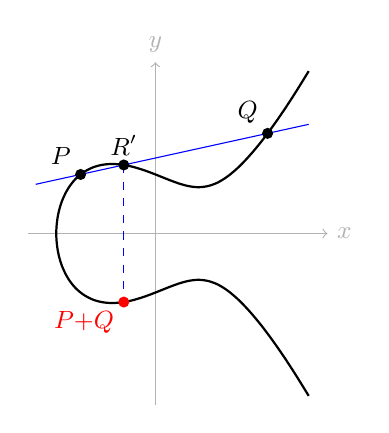
\begin{tikzpicture}[x=0.95cm, y=0.75cm, font=\small]
  \draw[gray!60, ->] (-1.7,0) -- (2.3,0) node[right] {$x$};
  \draw[gray!60, ->] (0,-2.9) -- (0,2.9) node[above] {$y$};
  \eccRealCurve
  \draw[blue] (-1.6,0.8331) -- (2.05,1.8486);
  \draw[blue, dashed] (-0.4226,1.1607) -- (-0.4226,-1.1607);
  \fill (-1,1) circle (2pt) node[above left] {$P$};
  \fill (1.5,1.6956) circle (2pt) node[above left] {$Q$};
  \fill (-0.4226,1.1607) circle (2pt) node[above] {$R'$};
  \fill[red] (-0.4226,-1.1607) circle (2pt) node[below left] {$P{+}Q$};
\end{tikzpicture}
\hfill
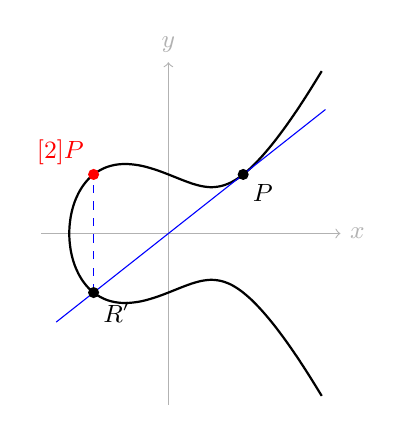
\begin{tikzpicture}[x=0.95cm, y=0.75cm, font=\small]
  \draw[gray!60, ->] (-1.7,0) -- (2.3,0) node[right] {$x$};
  \draw[gray!60, ->] (0,-2.9) -- (0,2.9) node[above] {$y$};
  \eccRealCurve
  \draw[blue] (-1.5,-1.5) -- (2.1,2.1);
  \draw[blue, dashed] (-1,-1) -- (-1,1);
  \fill (1,1) circle (2pt) node[below right] {$P$};
  \fill (-1,-1) circle (2pt) node[below right] {$R'$};
  \fill[red] (-1,1) circle (2pt) node[above left] {$[2]P$};
\end{tikzpicture}
\caption{The chord-and-tangent rule on the curve $y^2 = x^3 - x + 1$.
Left: the line through $P$ and $Q$ meets the curve at a third point $R'$,
and $P + Q$ is the reflection of $R'$.
Right: for doubling, the tangent line at $P = (1,1)$ meets the curve
again at $R' = (-1,-1)$, so $[2]P = (-1, 1)$.}
\label{fig:ecc-chord}
\end{figure}

\subsection{The addition formulas}

Turning the picture into algebra is a short calculation.
Let $P = (x_1, y_1)$ and $Q = (x_2, y_2)$ with $Q \neq -P$, and let
$y = \lambda x + \nu$ be the line through them (or the tangent at $P$
if $P = Q$), where $\nu = y_1 - \lambda x_1$.
Substituting the line into the curve equation gives
\[ (\lambda x + \nu)^2 = x^3 + ax + b
   \quad\Longleftrightarrow\quad
   x^3 - \lambda^2 x^2 + (a - 2\lambda\nu)x + (b - \nu^2) = 0. \]
This cubic has three roots: $x_1$, $x_2$, and the $x$-coordinate $x_3$ of
the third intersection point.
For a monic cubic, the sum of the roots is the negation of the
coefficient of $x^2$, so $x_1 + x_2 + x_3 = \lambda^2$.
That gives us $x_3$.
The third intersection point is $(x_3, \lambda x_3 + \nu)$,
and reflecting it gives $P + Q$.

The slope $\lambda$ is the slope of the chord through $P$ and $Q$, or,
when $P = Q$, the slope of the tangent, which we get by implicitly
differentiating $y^2 = x^3 + ax + b$ to obtain $2y \, dy = (3x^2 + a)\, dx$.
Putting everything together:

\begin{definition}[Elliptic-curve point addition]\label{defn:ecadd}
Let $P$ and $Q$ be points on the curve, possibly $\calO$.
For affine points, write $P = (x_1, y_1)$ and $Q = (x_2, y_2)$.
\begin{itemize}[noitemsep]
  \item If $P = \calO$, then $P + Q = Q$. If $Q = \calO$, then $P + Q = P$.
  \item If $x_1 = x_2$ and $y_1 = -y_2$, then $P + Q = \calO$.
  \item Otherwise, let
  \[ \lambda =
     \begin{cases}
       \dfrac{y_2 - y_1}{x_2 - x_1} & \text{if } P \neq Q,\\[2ex]
       \dfrac{3x_1^2 + a}{2y_1}     & \text{if } P = Q,
     \end{cases}
  \]
  and output $P + Q = (x_3, y_3)$, where
  \begin{align*}
    x_3 &= \lambda^2 - x_1 - x_2,\\
    y_3 &= \lambda(x_1 - x_3) - y_1.
  \end{align*}
\end{itemize}
\end{definition}

The second case covers both a vertical chord ($Q = -P$) and doubling a
point with $y_1 = 0$, where the tangent is vertical.
Notice that the formulas use the coefficient $a$ but \emph{never} the
coefficient $b$.
This innocent-looking fact will come back to haunt us in
\cref{sec:invalid-curve}.

\begin{theorem}
The points of an elliptic curve, together with $\calO$, form an abelian
group under the addition of Definition~\ref{defn:ecadd}, with identity $\calO$ and
inverse $-(x, y) = (x, -y)$.
\end{theorem}

Everything except associativity follows directly from the definition
(commutativity holds because the line through $P$ and $Q$ is the line
through $Q$ and $P$). Associativity has no short proof; see Silverman's
textbook.\autocite{Silverman09}

\section{Elliptic curves over finite fields}

To do cryptography, we need a \emph{finite} group whose elements we can
write down exactly.
So we replace the real numbers with the integers modulo a prime~$p$.

\paragraph{The field $\Fp$.}
For a prime $p$, the set $\Fp = \{0, 1, \dots, p-1\}$ with addition and
multiplication modulo $p$ is a \emph{field}: we can add, subtract, and
multiply, and we can divide by any non-zero element.
Division by $z \neq 0$ means multiplying by $z^{-1} \bmod p$, which we can
compute either with the extended Euclidean algorithm or as
$z^{-1} = z^{p-2} \bmod p$.
The second formula follows from Euler's theorem from the RSA chapter:
$\phi(p) = p - 1$, so $z \cdot z^{p-2} = z^{p-1} = 1 \bmod p$.

\begin{definition}[Elliptic curve over $\Fp$]
Let $p > 3$ be prime and let $a, b \in \Fp$ satisfy
$4a^3 + 27b^2 \neq 0 \bmod p$. The group of $\Fp$-points of the
elliptic curve $E \colon y^2 = x^3 + ax + b$ is
\[ E(\Fp) = \{ (x, y) \in \Fp \times \Fp \colon y^2 = x^3 + ax + b \bmod p \}
            \cup \{ \calO \}, \]
with the group operation given by the formulas of Definition~\ref{defn:ecadd},
where all arithmetic is done modulo $p$.
\end{definition}
\marginnote{We need $p > 3$ because the short Weierstrass form
$y^2 = x^3 + ax + b$ uses division by $2$ and $3$ when it is derived from
the general form. Curves over fields of characteristic $2$ or $3$ use
slightly different equations.}

The derivation of the addition formulas used only field operations,
so the same formulas define a group on $E(\Fp)$, even though the
``curve'' is now a scattered set of points (\cref{fig:ecc-f17}).

\subsection{A worked example}

Consider the curve
\[ E \colon y^2 = x^3 + 2x + 2 \quad \text{over } \F_{17}. \]
We have $4 \cdot 2^3 + 27 \cdot 2^2 = 140 = 4 \bmod 17 \neq 0$, so the
curve is non-singular.
To list its points, we can try each $x \in \F_{17}$ and check whether
$x^3 + 2x + 2$ is a square modulo $17$.
For example, $x = 5$ gives $125 + 10 + 2 = 137 = 1 \bmod 17$,
and $1 = 1^2 = 16^2 \bmod 17$, so $(5, 1)$ and $(5, 16)$ are on the curve.
Doing this for every $x$ gives $18$ points, plus $\calO$, for a total of
$|E(\F_{17})| = 19$.
Since $19$ is prime, Corollary~\ref{cor:primeorder} tells us that every point
other than $\calO$ generates the whole group.

\begin{marginfigure}
\centering
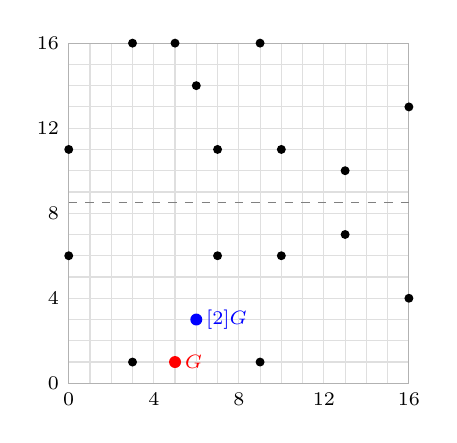
\begin{tikzpicture}[scale=0.27, font=\scriptsize]
  \draw[gray!25] (0,0) grid (16,16);
  \draw[gray!60] (0,0) rectangle (16,16);
  \foreach \t in {0,4,8,12,16} {
    \node[below] at (\t,0) {\t};
    \node[left] at (0,\t) {\t};
  }
  \draw[gray, dashed] (0,8.5) -- (16,8.5);
  \foreach \x/\y in {0/6,0/11,3/1,3/16,5/16,6/14,7/6,7/11,9/1,9/16,
                     10/6,10/11,13/7,13/10,16/4,16/13}
    \fill (\x,\y) circle (6pt);
  \fill[red] (5,1) circle (8pt) node[right] {$G$};
  \fill[blue] (6,3) circle (8pt) node[right] {$[2]G$};
\end{tikzpicture}
\caption{The $18$ affine points of $y^2 = x^3 + 2x + 2$ over $\F_{17}$
(the $19$th point, $\calO$, is not shown). The points are symmetric about
the dashed line $y = 17/2$, since $(x, y)$ and $(x, 17 - y) = (x, -y)$ are
both on the curve.}
\label{fig:ecc-f17}
\end{marginfigure}

\paragraph{Doubling.}
Let $G = (5, 1)$. To compute $[2]G$, we use the tangent formula:
\[ \lambda = \frac{3 \cdot 5^2 + 2}{2 \cdot 1} = \frac{77}{2} = 9 \cdot 2^{-1}
   = 9 \cdot 9 = 81 = 13 \bmod 17, \]
since $2 \cdot 9 = 18 = 1 \bmod 17$. Then
\begin{align*}
  x_3 &= 13^2 - 5 - 5 = 159 = 6 \bmod 17,\\
  y_3 &= 13 \cdot (5 - 6) - 1 = -14 = 3 \bmod 17,
\end{align*}
so $[2]G = (6, 3)$. You can check that $3^2 = 9 = 6^3 + 2 \cdot 6 + 2 \bmod 17$.

\paragraph{Adding.}
To compute $[3]G = G + [2]G = (5, 1) + (6, 3)$, we use the chord formula:
$\lambda = (3 - 1)/(6 - 5) = 2$, so
$x_3 = 4 - 5 - 6 = -7 = 10$ and $y_3 = 2(5 - 10) - 1 = -11 = 6 \bmod 17$,
and $[3]G = (10, 6)$.

Continuing in this way gives every multiple of $G$:

\begin{center}
\small\setlength{\tabcolsep}{4pt}
\begin{tabular}{rl@{\qquad}rl@{\qquad}rl}
\hline
$k$ & $[k]G$ & $k$ & $[k]G$ & $k$ & $[k]G$ \\
\hline
1 & $(5,1)$   & 7  & $(0,6)$   & 13 & $(16,4)$ \\
2 & $(6,3)$   & 8  & $(13,7)$  & 14 & $(9,1)$ \\
3 & $(10,6)$  & 9  & $(7,6)$   & 15 & $(3,16)$ \\
4 & $(3,1)$   & 10 & $(7,11)$  & 16 & $(10,11)$ \\
5 & $(9,16)$  & 11 & $(13,10)$ & 17 & $(6,14)$ \\
6 & $(16,13)$ & 12 & $(0,11)$  & 18 & $(5,16)$ \\
\hline
\end{tabular}
\end{center}

\noindent and $[19]G = \calO$.
Notice that $[19 - k]G = -[k]G$, and that the multiples of $G$ jump
around the grid with no apparent pattern: given $(16, 4)$, the only
obvious way to find $k$ with $[k]G = (16, 4)$ is to look it up in the
table. For a group with $2^{256}$ elements, there is no table.

\subsection{How many points are on a curve?}

Roughly half of the values $x \in \Fp$ make $x^3 + ax + b$ a square,
giving two points $(x, \pm y)$ each, so we expect about $p$ points.

\begin{theorem}[Hasse]
For an elliptic curve $E$ over $\Fp$,
\[ \big|\, |E(\Fp)| - (p + 1) \,\big| \le 2\sqrt{p}. \]
\end{theorem}

So a curve over a $256$-bit prime field has about $2^{256}$ points,
and Schoof's algorithm\autocite{Schoof85} computes the exact number in
time polynomial in $\log p$, which makes it possible to search for curves
of prime order.
For cryptography, we want the group order to be a large prime $n$, or
at least $|E(\Fp)| = h \cdot n$ for a large prime $n$ and a small
\emph{cofactor} $h$.
We then fix a \emph{base point} $G$ of order $n$ and work in the cyclic
subgroup $\langle G \rangle = \{\calO, G, [2]G, \dots, [n-1]G\}$.
For the NIST curve P-256, $h = 1$; for Curve25519, $h = 8$.

\paragraph{Point compression.}
\label{sec:compression}
\marginnote{Decompressing requires a square root modulo $p$. When
$p \equiv 3 \pmod 4$, as for P-256, and $z = w^2$ is a square, then
$y = z^{(p+1)/4}$ works, since $y^2 = z \cdot z^{(p-1)/2} = z \cdot
w^{p-1} = z \bmod p$ by Euler's theorem.}
Given $x$, the only possible $y$ values are the two square roots $\pm y$ of
$x^3 + ax + b$, and exactly one of $y$ and $p - y$ is even.
So a point can be stored as its $x$-coordinate plus one parity bit:
$33$ bytes for P-256.

\section{Scalar multiplication}
\label{sec:scalarmult}

The elliptic-curve analogue of computing $g^x$ is computing $[k]P$ for a
scalar $k$ of about $256$ bits.
Adding $P$ to itself $k$ times would take $2^{256}$ steps, but we can use
the same trick as in square-and-multiply exponentiation.
For $k = 0$, return $\calO$. For $k > 0$, write $k$ in binary as $k = (k_{\ell-1} k_{\ell-2} \cdots k_0)_2$ with
$k_{\ell-1} = 1$, and process the bits from most to least significant:

\begin{itemize}
  \item $\mathsf{ScalarMult}(k, P) \to [k]P$. (Double-and-add.)
  \begin{itemize}[noitemsep]
    \item If $k = 0$, output $\calO$ and stop.
    \item Set $R \gets P$.
    \item For $i = \ell - 2$ down to $0$:
    \begin{itemize}[noitemsep]
      \item $R \gets [2]R$.
      \item If $k_i = 1$, set $R \gets R + P$.
    \end{itemize}
    \item Output $R$.
  \end{itemize}
\end{itemize}

\marginnote{The formulas of Definition~\ref{defn:ecadd} need a field inversion for
every group operation, and inversions are much slower than
multiplications. Real implementations represent points in
\emph{projective coordinates} $(X : Y : Z)$, which stand for
$(X/Z, Y/Z)$, and perform a single inversion at the very end.}
\marginnote{Projective coordinates also give the point at infinity a
concrete form. Substituting $x = X/Z$ and $y = Y/Z$ into the curve
equation and clearing denominators gives
$Y^2 Z = X^3 + aXZ^2 + bZ^3$. Setting $Z = 0$ forces $X = 0$, so
$\calO = (0 : 1 : 0)$ is the only point with $Z = 0$. Every vertical
line $X = cZ$ passes through it. In code, checking that $P \neq \calO$
means checking that $Z \neq 0$. A point received as an affine pair
$(x, y)$ that satisfies the curve equation can never be $\calO$; the
SEC~1 encoding represents $\calO$ by the single byte \texttt{0x00}.}
Doubling appends a $0$ bit to the scalar and adding $P$ turns it into a
$1$; for example, $7 = (111)_2$, so $[7]G$ is computed as
$G \to [2]G \to [3]G \to [6]G \to [7]G$.
Double-and-add takes at most $2\ell$ group operations, each costing a
handful of multiplications in $\Fp$.

\paragraph{Side channels.}
Double-and-add performs an extra addition exactly when a bit of $k$ is
$1$, so an attacker who can measure its timing or power consumption can
read off a secret~$k$, as in the side-channel chapter.
Real implementations use constant-time algorithms such as the
\emph{Montgomery ladder}, which does one doubling and one addition per
bit regardless of its value.

\section{The elliptic-curve discrete-log problem}
\label{sec:ecdlp}

We can now state the assumption on which all of elliptic-curve
cryptography rests.
Fix a curve $E$ over $\Fp$ and a base point $G \in E(\Fp)$ of prime order~$n$.

\begin{definition}[Elliptic-curve discrete-log (ECDLP) assumption]
For all efficient adversaries $\calA$:
\[ \Pr\left[\calA(G, [x]G) = x \colon x \getsr \{0, 1, \dots, n-1\}\right]
   \leq \negl. \]
\end{definition}

\marginnote{On some special curves, the ECDDH assumption is
\emph{false} even though ECCDH and ECDLP appear hard: a ``pairing'' on
the curve lets anyone test whether a tuple has the Diffie-Hellman form.
Such pairing-friendly curves are useful for advanced constructions such
as short BLS signatures, but they are never used for plain ElGamal.}
Likewise, ECCDH says that given $(G, [x]G, [y]G)$ it is infeasible to
compute $[xy]G$, and ECDDH says that for $x, y, z \getsr \{0, \dots, n-1\}$,
the tuples $(G, [x]G, [y]G, [xy]G)$ and $(G, [x]G, [y]G, [z]G)$ are
computationally indistinguishable.

\subsection{Elliptic-curve Diffie-Hellman}

Elliptic-curve Diffie-Hellman (ECDH) is the Diffie-Hellman protocol in
additive notation.
The public parameters are the curve $E$, the prime $p$, and a base point
$G$ of prime order $n$.

\begin{itemize}[noitemsep]
  \item $\Gen() \to (\sk, \pk)$.
    \begin{itemize}[noitemsep]
      \item Sample $\sk \getsr \{1, \dots, n-1\}$.
      \item Set $\pk \gets [\sk]G \in E(\Fp)$.
      \item Output $(\sk, \pk)$.
    \end{itemize}
  \item $\mathsf{Derive}(\sk_A, \pk_B) \to k$.
    \begin{itemize}[noitemsep]
      \item Check that $\pk_B$ is a valid point in $\langle G\rangle$
            and $\pk_B \neq \calO$; otherwise output $\bot$.
      \item Output $k \gets [\sk_A]\pk_B \in E(\Fp)$.
    \end{itemize}
\end{itemize}

\paragraph{Correctness.}
If $\pk_A = [a]G$ and $\pk_B = [b]G$, then
\[ [a]\pk_B = [a]([b]G) = [ab]G = [ba]G = [b]([a]G) = [b]\pk_A. \]
In practice, the parties hash the shared point (usually its
$x$-coordinate) to obtain a symmetric key, as over $\Z^*_p$.

\subsection{How hard is the ECDLP?}

\paragraph{Generic attacks.}
\marginnote{Pollard's rho algorithm takes a pseudorandom walk through the
group in which each step is a known combination $[\alpha]G + [\beta]Q$.
After about $\sqrt{\pi n / 2}$ steps in the idealized random-walk model, by the birthday paradox, the walk
revisits a point, which gives an equation
$[\alpha]G + [\beta]Q = [\alpha']G + [\beta']Q$ that can be solved
for~$x$ provided $\beta-\beta' \neq 0 \bmod n$; otherwise the
attempt must be retried.}
Some discrete-log algorithms work in \emph{any} group.
\emph{Baby-step giant-step} writes $x = im + j$ with
$m = \lceil \sqrt{n} \rceil$, stores $[j]G$ for all $j < m$ in a table,
and then computes $Q - [im]G$ for $i = 0, 1, \dots$ until it finds a
match, using about $\sqrt{n}$ time and memory.
Pollard's rho algorithm\autocite{Pollard78} achieves the same
$O(\sqrt{n})$ running time with only a constant amount of memory, and it
parallelizes well, so it is the algorithm used in practice to attack
elliptic curves.

Shoup proved that no generic algorithm can do better than
$\Omega(\sqrt{n})$,\autocite{Shoup97} so on a curve of $256$-bit prime
order, generic attacks take about $2^{128}$ operations.
\marginnote{The largest elliptic-curve discrete-log instances solved in
public are around $112$ to $117$ bits.}

\paragraph{Why we use a large prime-order subgroup.}
If the order of $G$ is $n = n_1 n_2$ with $\gcd(n_1, n_2) = 1$, then
$[n_2]G$ has order $n_1$ and $[n_2]Q = [x]([n_2]G)$, so a discrete log in
the small subgroup of order $n_1$ reveals $x \bmod n_1$. Doing the same
for $n_2$ and combining with the Chinese Remainder Theorem gives $x$.
This \emph{Pohlig-Hellman} algorithm\autocite{PohligHellman78} runs in
time governed by the \emph{largest prime factor} of $n$, which is why $G$
should be chosen to generate a large prime-order subgroup.

\paragraph{No Number Field Sieve.}
The sub-exponential attacks on $\Z^*_p$ view group elements as integers
and exploit the fact that integers often factor into small primes.
Points on an elliptic curve have no useful analogue of factoring into
``small'' points, as Miller observed in his original
proposal.\autocite{Miller85}
More than forty years later, for well-chosen curves over prime fields, the
best known attacks are still the generic $\sqrt{n}$ ones.

\section{Choosing a curve}

Not every elliptic curve is a good one. Discrete log is easy on
\emph{singular} curves ($4a^3 + 27b^2 = 0$), on \emph{anomalous} curves
with $|E(\Fp)| = p$,\autocite{Smart99} and is reduced to discrete log in
a finite field $\F_{p^k}$ (where the Number Field Sieve applies) on curves
whose group order $n$ divides $p^k - 1$ for small~$k$, such as
supersingular curves.\autocite{MOV93}
So almost all applications use one of a few standardized curves.
\textbf{P-256}, standardized by NIST, is
$y^2 = x^3 - 3x + b$ over $p = 2^{256} - 2^{224} + 2^{192} + 2^{96} - 1$,
with prime order.
\textbf{Curve25519}, designed by Bernstein,\autocite{Bernstein06} is
$y^2 = x^3 + 486662x^2 + x$ over $p = 2^{255} - 19$, with order $8\ell$
for a prime $\ell \approx 2^{252}$; this ``Montgomery'' form allows a fast
constant-time ladder that uses only $x$-coordinates.
\textbf{secp256k1}, used by Bitcoin, is $y^2 = x^3 + 7$ over
$p = 2^{256} - 2^{32} - 977$.

\paragraph{Can we trust the curve?}
The constant $b$ in P-256 is derived from a published seed using SHA-1,
not simply equal to a hash output. The derivation constructs an integer
$c$ from hash outputs and chooses $b$ satisfying $b^2c = -27 \bmod p$.
This makes the derivation verifiable, but does not explain how the seed
itself was chosen.
No weakness has ever been found, and P-256 is believed to be secure.
\marginnote{This concern is not entirely paranoid. The Dual EC DRBG
pseudorandom generator, standardized by NIST in 2006, used two
elliptic-curve points of unexplained origin; documents leaked in 2013
indicated that it had been deliberately weakened, and NIST withdrew it in
2014.}
Curve25519 is \emph{rigid}: every parameter is the simplest choice
satisfying published criteria, leaving no freedom to hide a backdoor.

\section{Pitfall: Invalid-curve attacks}
\label{sec:invalid-curve}

Recall that the addition formulas in Definition~\ref{defn:ecadd} never use the
coefficient $b$.
So if an implementation receives a point $P' = (x', y')$ from the network
and multiplies it by its secret key without checking that $P'$ lies on
the curve, it computes $[\sk]P'$ correctly on \emph{whatever curve}
$y^2 = x^3 + ax + b'$ the point happens to satisfy, where
$b' = y'^2 - x'^3 - ax'$.

An attacker can exploit this by choosing $b'$ so that the curve
$E' \colon y^2 = x^3 + ax + b'$ has a point $P'$ of some small prime order
$\ell$, and sending $P'$ in place of a legitimate public key or
ciphertext component.
The victim's $S = [\sk]P' = [\sk \bmod \ell]P'$ takes only $\ell$
possible values, and the attacker can usually tell which one occurred,
for example by checking which candidate key decrypts the victim's next
message. This reveals $\sk \bmod \ell$.
Repeating with points of different small prime orders until their product
exceeds $n$ and applying the Chinese Remainder Theorem gives $\sk$.
This is the Pohlig-Hellman idea again, applied to a group that the
attacker chose.
Invalid-curve attacks have broken real systems, including several TLS
libraries\autocite{JSS15} and the Bluetooth pairing protocol, whose
specification did not require devices to validate the public keys they
received.\autocite{BihamNeumann19}

\paragraph{\textbf{IMPORTANT}:}
For the full-point protocols here, validate received point encodings and
check curve membership before using them. Public keys and ephemeral DH
components must not be $\calO$. If the curve has a cofactor $h > 1$,
these DH inputs must also lie in the subgroup of order $n$, unless the
protocol is specifically designed to be safe without this check.
Nonidentity requirements depend on the point's role: textbook ElGamal's
$C_2$ may legitimately equal $\calO$, for example when $M = -[r]A$.
\marginnote{X25519 avoids explicit full-point curve-membership checks:
its $x$-coordinate inputs correspond to Curve25519 or its quadratic
twist, both with large prime-order subgroups. Clamping makes the scalar
a multiple of $8$, eliminating small-order components. A purely
small-order input nevertheless yields an all-zero shared secret.
Protocols requiring rejection of this predictable secret, including
HPKE, must check for an all-zero output and abort.}

\section{ElGamal encryption on elliptic curves}

We present two versions of elliptic-curve ElGamal. The ``textbook''
version encrypts a message that is itself a point and shows the structure
most clearly. The ``hashed'' version is the analogue of hashed ElGamal
over $\Z^*_p$, and is the one used in practice.

Throughout, the public parameters are a curve $E$ over $\Fp$ and a base
point $G$ of prime order $n$.
For the textbook scheme, we assume for simplicity that
$|E(\Fp)| = n$ is itself prime (cofactor $h = 1$), so every point on the
curve is in $\langle G \rangle$.

\subsection{Textbook elliptic-curve ElGamal}

\begin{definition}[Textbook EC ElGamal]
The message space is $\calM = E(\Fp)$.
\begin{itemize}
  \item $\Gen() \to (\sk, \pk)$:
    \begin{itemize}[noitemsep]
      \item Choose $a \getsr \{1, \dots, n-1\}$.
      \item Compute $A \gets [a]G$.
      \item Output $(\sk, \pk) \gets (a, A)$.
    \end{itemize}
  \item $\Enc(\pk, M) \to (C_1, C_2)$:
    \begin{itemize}[noitemsep]
      \item Check that $A$ is a valid point in $\langle G\rangle$
            and $A \neq \calO$; otherwise output $\bot$.
      \item Choose $r \getsr \{1, \dots, n-1\}$.
      \item Compute $C_1 \gets [r]G$.
      \item Compute $C_2 \gets M + [r]A$.
      \item Output $(C_1, C_2)$.
    \end{itemize}
  \item $\Dec(\sk, (C_1, C_2)) \to M$:
    \begin{itemize}[noitemsep]
      \item Check that $C_1$ and $C_2$ are points on $E$ and that
            $C_1 \neq \calO$; if not, output $\bot$.
      \item Compute $S \gets [a]C_1$.
      \item Output $M \gets C_2 - S$.
    \end{itemize}
\end{itemize}
\end{definition}

The sender runs a Diffie-Hellman key exchange on the fly:
$C_1 = [r]G$ is a fresh, single-use Diffie-Hellman public key, and
$S = [r]A = [ra]G$ is the shared point, which she adds to the message as a
``one-time pad'' in the group. The recipient subtracts it off, where
$C_2 - S = C_2 + (-S)$ and $-S$ is $S$ with its $y$-coordinate negated.

\paragraph{Correctness.}
Let $A = [a]G$, and let $(C_1, C_2) = ([r]G,\ M + [r]A)$ be an encryption
of $M$. Decryption computes
\[ C_2 - [a]C_1
   \;=\; M + [r]([a]G) - [a]([r]G)
   \;=\; M + [ra]G - [ar]G
   \;=\; M. \]
As with Diffie-Hellman, all we used is that $ra = ar$, so correctness
holds for every choice of $a$ and $r$.

\paragraph{A worked example.}
Let us encrypt on the toy curve $y^2 = x^3 + 2x + 2$ over $\F_{17}$ with
$G = (5, 1)$ and $n = 19$, using the table of multiples of $G$ from
earlier.
\begin{itemize}
  \item \textbf{Key generation.} The recipient chooses $a = 7$ and
        publishes $A = [7]G = (0, 6)$.
  \item \textbf{Encryption.} The sender wants to encrypt the point
        $M = (9, 1)$. She chooses $r = 10$ and computes
        $C_1 = [10]G = (7, 11)$ and the shared point
        $S = [10]A = [70]G = [13]G = (16, 4)$, since $70 = 13 \bmod 19$.
        Then $C_2 = M + S = (9, 1) + (16, 4)$. Modulo $17$,
        \begin{align*}
          \lambda &= (4 - 1)/(16 - 9) = 3 \cdot 7^{-1} = 3 \cdot 5 = 15,\\
          x_3 &= 15^2 - 9 - 16 = 13, \quad y_3 = 15(9 - 13) - 1 = 7.
        \end{align*}
        The ciphertext is $(C_1, C_2) = \big((7, 11), (13, 7)\big)$.
  \item \textbf{Decryption.} The recipient computes
        $S = [7]C_1 = [7]([10]G) = [70]G = (16, 4)$, so $-S = (16, 13)$.
        Then $C_2 - S = (13, 7) + (16, 13)$:
        \begin{align*}
          \lambda &= (13 - 7)/(16 - 13) = 2,\\
          x_3 &= 4 - 13 - 16 = 9, \quad y_3 = 2(13 - 9) - 7 = 1,
        \end{align*}
        which recovers $M = (9, 1)$.
\end{itemize}
Note that the recipient never needed to know that $M = [14]G$; neither
party has to solve a discrete log.

\paragraph{Encoding messages as points.}
To encrypt a bit string, first encode it reversibly as a nonnegative
integer $m$ (preserving its length). Choose a positive integer $K$ and
restrict $0 \le m < \lfloor p/K \rfloor$.
Koblitz's method\autocite{Koblitz87} tries $x = mK + j$ for
$j = 0, 1, \dots, K-1$ until $x^3 + ax + b$ is a square and takes $y$ to be
one of its square roots. The bound ensures $x < p$, so decoding recovers
$m = \lfloor x/K \rfloor$ without modular wraparound.
If no candidate works, encoding fails. Treating the square tests as
independent trials suggests a failure rate of about $2^{-K}$; this is a
heuristic, not a guarantee for every fixed message and curve.
Hashed ElGamal, below, avoids the issue entirely.

\paragraph{Security.}
Textbook EC ElGamal is secure against chosen-plaintext attacks under the
ECDDH assumption.
The intuition is that the adversary sees $(G, A, C_1, C_2) =
(G, [a]G, [r]G, M + [ar]G)$.
By ECDDH, this is indistinguishable from $(G, [a]G, [r]G, M + [z]G)$ for
a uniformly random $z$.
But $[z]G$ is a uniformly random point that is independent of $M$, so
$M + [z]G$ is also a uniformly random point that reveals nothing about
$M$, exactly as with a one-time pad.

\marginnote{Malleability is sometimes a feature. In ``exponential''
ElGamal, a small integer $m$ is encrypted as the point $[m]G$, and adding
two ciphertexts component-wise gives an encryption of $[m + m']G$.
Electronic-voting systems use this to add up encrypted votes, decrypting
only the final tally, which is small enough that its discrete log can be
found by brute force.}
Textbook ElGamal is \emph{not} secure against chosen-ciphertext attacks,
however, because it is \emph{malleable}.
Given an encryption $(C_1, C_2)$ of an unknown $M$, anyone can choose
$M' \neq \calO$ and produce $(C_1, C_2 + M')$, which is a valid encryption
of $M + M'$.
An adversary in the CCA game can submit this modified ciphertext to the
decryption oracle (it is not equal to the challenge ciphertext), subtract
$M'$ from the answer, and recover~$M$.

\subsection{Hashed elliptic-curve ElGamal}

Hashed ElGamal fixes both problems with the textbook scheme: it encrypts
arbitrary bit strings, and it is secure against chosen-ciphertext attacks.
Instead of using the shared point $S$ as a one-time pad, it hashes $S$ to
a symmetric key and encrypts the message with an authenticated-encryption
scheme.
The construction is identical to hashed ElGamal over $\Z^*_p$; only the
group has changed.
\marginnote{Here $H$ must use a canonical, injective point encoding,
such as the full compressed encoding including the parity bit.
Hashing only the $x$-coordinate is insecure in this construction:
$(R,c')$ and $(-R,c')$ would decrypt under the same key, giving a
chosen-ciphertext attack. Practical constructions also bind the
encapsulation and recipient public key into key derivation.}

\begin{definition}[Hashed EC ElGamal]
Let $H \colon E(\Fp) \to \calK'$ be a hash function (modeled as a random
oracle) and let $(\Enc', \Dec')$ be an authenticated-encryption scheme
with key space $\calK'$ and message space $\calM = \zo^*$.
Represent every transmitted point by its unique canonical encoding and
reject noncanonical encodings; evaluate $H$ on the full point encoding.
\begin{itemize}
  \item $\Gen() \to (\sk, \pk)$:
    \begin{itemize}[noitemsep]
      \item Choose $a \getsr \{1, \dots, n-1\}$.
      \item Compute $A \gets [a]G$.
      \item Output $(\sk, \pk) \gets (a, A)$.
    \end{itemize}
  \item $\Enc(\pk, m) \to c$:
    \begin{itemize}[noitemsep]
      \item Check that $A$ is a valid point in $\langle G\rangle$
            and $A \neq \calO$; otherwise output $\bot$.
      \item Choose $r \getsr \{1, \dots, n-1\}$.
      \item Compute $R \gets [r]G$.
      \item Compute $k \gets H([r]A)$.
      \item Output $c \gets (R, \Enc'(k, m))$.
    \end{itemize}
  \item $\Dec(\sk, c) \to m$:
    \begin{itemize}[noitemsep]
      \item Parse $(R, c') \gets c$.
      \item Check that $R$ is a point on $E$, that $R \neq \calO$, and
            that $R$ lies in $\langle G \rangle$; if not, output $\bot$.
      \item Compute $k \gets H([a]R)$.
      \item Output $m \gets \Dec'(k, c')$.
    \end{itemize}
\end{itemize}
\end{definition}


\paragraph{Correctness.}
The sender computes $k = H([r]A) = H([ra]G)$ and the recipient computes
$k' = H([a]R) = H([ar]G)$.
These are equal, so
$\Dec(\sk, c) = \Dec'(k', \Enc'(k, m)) = \Dec'(k, \Enc'(k, m)) = m$
by the correctness of the authenticated-encryption scheme.
An honestly generated $R = [r]G$ always passes the validity check.

\paragraph{Security.}
Modeling $H$ as a random oracle on full, canonically encoded points,
hashed EC ElGamal is secure against chosen-ciphertext attacks under the
\emph{strong DH} assumption and the security of the authenticated-encryption
scheme $(\Enc', \Dec')$. Here strong DH means that, given $A=[a]G$ and
$R=[r]G$, computing $[ar]G$ remains hard even with an oracle that, on
inputs $(U,V)$, tests whether $V=[a]U$. The stronger Gap-CDH assumption,
which grants a general DDH oracle, also suffices. Plain ECCDH hardness
alone does not supply the standard CCA proof.\footnote{See David Cash,
Eike Kiltz, and Victor Shoup, ``The Twin Diffie-Hellman Problem and
Applications,'' EUROCRYPT 2008, Section 1.}
For nonzero $a$, distinct subgroup points $R$ give distinct shared points;
full-point hashing avoids the sign ambiguity described in the margin.
The security proof must also account for adaptive decryption queries,
which is why the strengthened DH assumption is needed.
Note the validity check on $R$, though: the proof assumes
$R \in \langle G \rangle$, and without the check the decryption oracle is
exactly the oracle that the invalid-curve attack of
\cref{sec:invalid-curve} needs to recover the secret key~$a$.

\paragraph{In practice.}
This scheme is known as ECIES, and a modern version of it is the core
of HPKE,\autocite{HPKE} used in TLS's Encrypted Client Hello, typically
with X25519, HKDF-SHA256, and AES-GCM.
Encryption takes two scalar multiplications ($[r]G$, which can use a
precomputed table, and $[r]A$); decryption takes one ($[a]R$). Each takes
tens of microseconds, versus about a millisecond for an exponentiation
modulo a $3072$-bit prime, depending on the implementation and hardware.
The encapsulation uses $32$ bytes with X25519. A compressed P-256 point
uses $33$ bytes, but HPKE specifies an uncompressed P-256 encoding and
therefore uses $65$ bytes. These are encapsulation sizes only, excluding
the authenticated-encryption overhead, compared with a $384$-byte field
element for a $3072$-bit finite-field instantiation.
